Wintertodt is a skilling boss that is primarily fought (in a manner similar to a minigame moreso than combat) for firemaking experience and resources, either solo or as part of a (large) group. Experience is gained from actions during the fight, with a bonus awarded for players that have contributed enough. The bonus provides experience and supply crates which contain valuable resources.

\begin{figure}
	\centering
	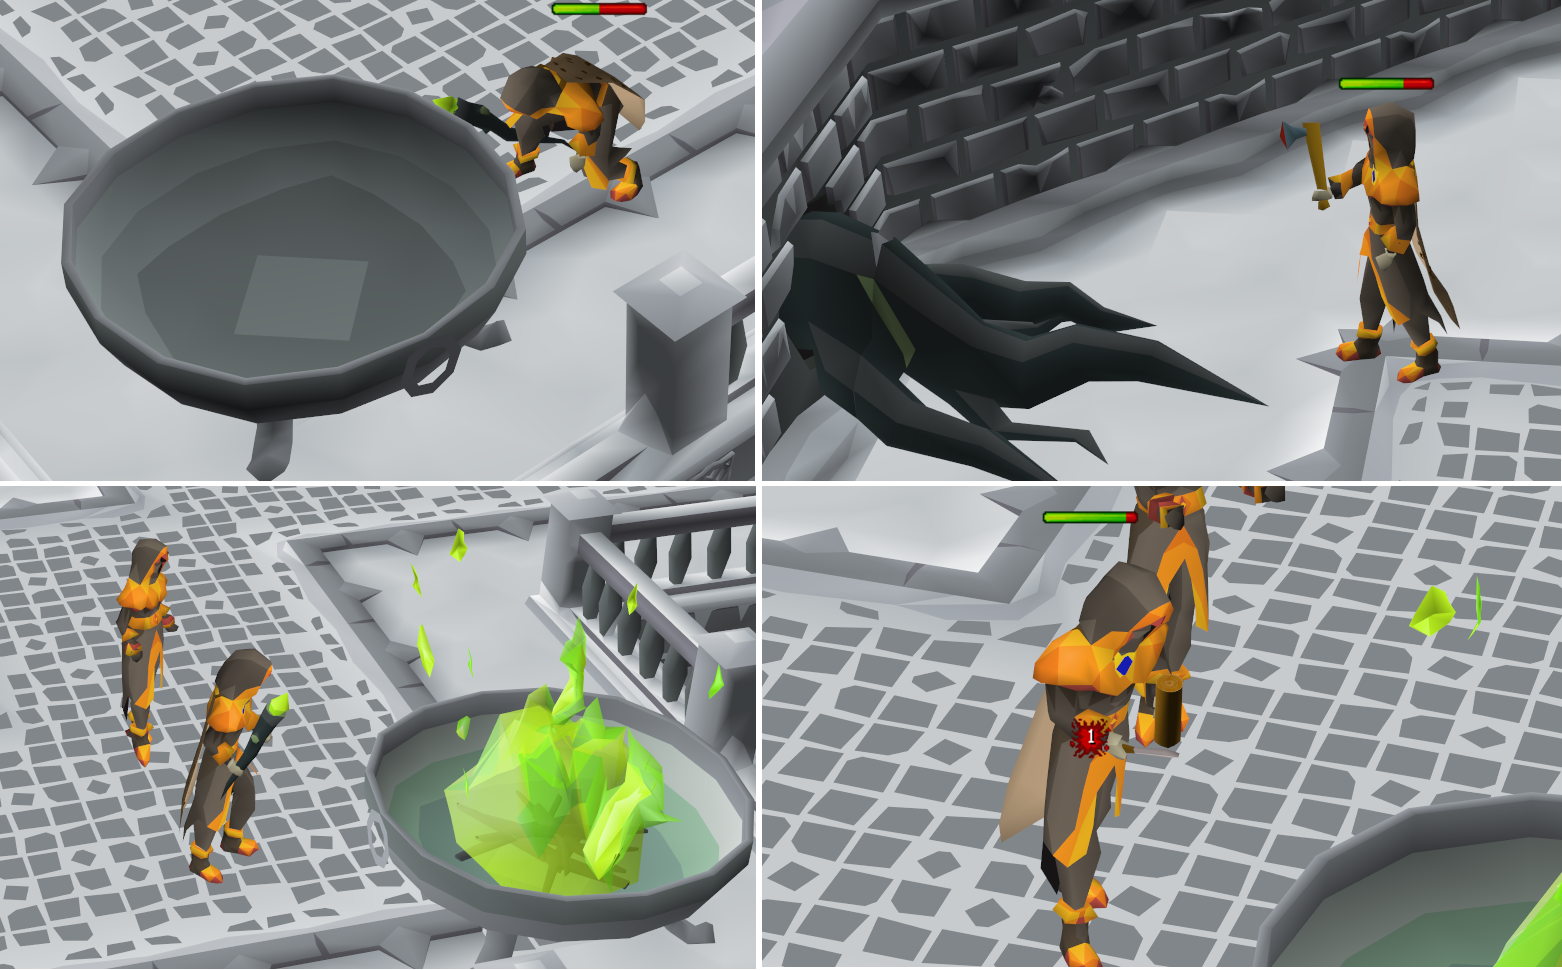
\includegraphics[width=\linewidth]{img/firemaking/wintertodt_actions.png}
	\caption{
		A player performing several actions during a Wintertodt fight. From top-left to bottom-right the player is: lighting a brazier, chopping tree roots, burning roots/kindling, and fletching roots into kindling. Actions that are not shown including creating potions, healing the Pyromancer, and fixing/repairing the brazier.
	}
	\label{fig:wintertodt_actions}
\end{figure}

The objective of the fight is to defeat the Wintertodt. This boss takes damage over time while any of the four braziers in the room are lit. Actions that the player performs are centered on maintaining and feeding these braziers. Feeding the braziers provides the majority of the firemaking experience. They are occasionally extinguished (by the cold wind), and broken (by the flame's heat). Additionally the Pyromancer associated with each brazier may need healing before a player can relight an extinguished brazier. In a group fight, the maintenance actions can be performed by others. To feed the braziers, players will chop Bruma roots and optionally fletch them into kindling. This provides more experience and points when burned, but requires more time to process. Several of these actions are shown in Fig.~\ref{fig:wintertodt_actions}.

Most of these actions award the player with points and provide experience in some skill. The experience scales linearly with the respective skill level, with the proportionality constant, $M$, determined by the action. If the player reaches a threshold of 500 points, they gain bonus experience and a supply crate at the end of a fight. A summary of these actions can be found below in Table.~\ref{table:wintertodt_actions}.


\begin{table}[H]
	\caption{Actions and the associated skills, XP multipliers, and points awarded.}
	\centering
	\begin{tabular}{lcccc}
		\multicolumn{1}{c}{\textbf{Action}} & \textbf{Skill}                                                                   & \textbf{XP Multiplier} ($M$) & \textbf{Points} \\
		Lighting braziers                   & 
\includegraphics[width=0.03\linewidth]{img/general/skills/Firemaking_icon.png}   & 6.0x                     & 25              \\
		Chopping Root                       & 
\includegraphics[width=0.03\linewidth]{img/general/skills/Woodcutting_icon.png}  & 0.3x                   & -               \\
		Burning Root                        & 
\includegraphics[width=0.03\linewidth]{img/general/skills/Firemaking_icon.png}   & 3.0x                     & 10              \\
		Burning Kindling                    & 
\includegraphics[width=0.03\linewidth]{img/general/skills/Firemaking_icon.png}   & 3.8x                   & 25              \\
		Repairing Brazier                   & 
\includegraphics[width=0.03\linewidth]{img/general/skills/Construction_icon.png} & 4.0x                     & 25              \\
		Healing Pyromancer                  & 
\includegraphics[width=0.03\linewidth]{img/general/skills/blank.png}             & 0.1x                   & 30              \\
		Creating Potion                     & 
\includegraphics[width=0.03\linewidth]{img/general/skills/Herblore_icon.png}     & -                      & -               \\
		Picking Bruma Herb                  & 
\includegraphics[width=0.03\linewidth]{img/general/skills/Farming_icon.png}      & -                      & -               \\
		Win with 500+ Points                & 
\includegraphics[width=0.03\linewidth]{img/general/skills/Firemaking_icon.png}   & 100x                   & -              
	\end{tabular}
	\label{table:wintertodt_actions}
\end{table}

There are several problems that would be interesting to solve. The mechanics to model and important problems vary depending on whether the boss is fought in a large group or solo. For solo fights, the optimal strategy (i.e. which actions to perform when) could be investigated. For large groups, we can ignore the emergent behavior of the players by making certain assumptions. For example, the root chopping rate can be ignored if we assume that the player always reaches a target number of points. We will tackle the latter since group fights are (empirically) more common. The quantities of interest are the number of kills required to obtain a certain level, the number of crates/value/resources obtained after a certain number of kills, and the time required for a kill. We will only be concerned with firemaking experience for now.

\section{Large groups}
	We will be attempting to determine the number of games required to get to a desired firemaking level. Since the game play is relatively involved, we will apply a constraint to the player's actions to make it more manageable. We will limit the actions to: burning, fletching, and cutting (so ignoring: healing, relighting, and repairing). Although this isn't exactly how players would play, relighting is the only action that provides firemaking experience, and all ignored actions can be performed by other players. Furthermore, all those actions are infrequent in comparison to burning and so these shouldn't be too significant.

	Let $M_\text{root}=3$, $M_\text{kindling}=3.8$, and $M_\text{bonus}=100$ be the XP multiplier for burning a root, burning a kindling, and obtaining 500+ points, respectively. We also have that $P_\text{root}=10$ points are given for burning a root, and $P_\text{kindling}=25$ are given for burning kindling. Since the player may level up during a fight (and thereby change their experience rate), we consider this problem in two stages: within a fight and across fights. Finally, we will need to make use of the level equation, $\mathcal{L}$ from Chapter~\ref{chp:experience_and_levels}, that tells us what level a skill is, given its experience.

	\subsection{Within a Fight}
		Since a player may level up over the course of a fight, we need to consider the experience gained on a per action basis. We will label the total player's firemaking experience after $a$ actions are performed as $E_a$. The firemaking actions during a fight come from burning either roots or kindling. To be general, let's define an indicator function $\delta^n_\text{action}$ that is 1 if the $n$'th action performed by the player matches the subscripted value, and is zero otherwise. For example, $\delta^n_\text{root}=1$ if the $n$'th action was burning a root. Then, the value of the XP multiplier for the $n$'th firemaking action can be defined as:
		\begin{align}
			c_n \equiv \delta_\text{root}^n M_\text{root} + \delta_\text{kindling}^n M_\text{kindling}.
		\end{align}
		Starting with $E_0$ experience, the experience after $a$ actions during a kill is governed by:
		\begin{align}
			E_{n+1} &= E_{n} + c_n\mathcal{L}(E_{n})
		\end{align}
		This equation \emph{may} have a solution except that $\mathcal{L}$ has no analytic form, and so this must be evaluated iteratively. Practically, we can introduce player policies or strategies, that model how a player acts, by labeling the coefficients as $c_n^\text{policy}$. A policy essentially generates the sequence of player actions, for example: an \emph{Only Burning Roots} (OBR) policy could be defined as:
		\begin{align}
			c_n^\text{OBR} \equiv \begin{cases}
				M_\text{root} & \text{if } n \le T/P_\text{root}\\
				0 & \text{otherwise}.
			\end{cases}
		\end{align}
		Regarding notation, the labeling $E_{n}^\text{policy}$ may now be used to denote the experience gained according to some policy. More advanced policies can also be defined. A reasonable strategy to maximize experience while reaching the point threshold would be to burn kindling until the player obtains 500 points followed by burning logs until they reach some target number of points, $T$. We can call this the \emph{Kindle Till Bonus} (KTB) policy, which could be defined as:
		\begin{align}
			c_n^\text{KTB} \equiv \begin{cases}
				M_\text{kindling} &\text{if } n \le 500/P_\text{kindling}\\
				M_\text{root} &\text{if } n \le \frac{T}{P_\text{root}} - \frac{P_\text{kindling}}{P_\text{root}}\lceil 500/P_\text{kindling} \rceil \\
				0 & \text{otherwise}.
			\end{cases}
		\end{align}
		The first bound is the number of kindling needed to reach 500 points. The second bound is the number of points remaining, divided by the points per root which gives the number of roots left.


	\subsection{Across Fights}
		We now have the ability to calculate the firemaking experience gained during a fight. We can take this further to calculate the firemaking experience gained across fights. The experience that a player has after $k$ kills can be denoted as $\mathcal{E}^k$. There are two contributions for this: one is the experience that a player gains during a fight, the other is the bonus experience gained after a kill. And so,
		\begin{align}\label{eq:experience_over_kills}
			\mathcal{E}^{k+1} &= \mathcal{E}^k + E_{N(T; \text{policy})}^\text{policy} + \theta(T - 500)M_\text{bonus}\mathcal{L}(\mathcal{E}^k),
		\end{align}
		where $N(T; \text{policy})$ is the number of actions to perform given the target and policy, and $\theta$ is the Heaviside step function. This equation can, again, only be evaluated numerically. 

	\subsection{Kill Count, Time to Level, and Reward Value}
		Equation~(\ref{eq:experience_over_kills}) can be used to calculate the experience gained after a certain amount of kills. Programmatically inverting this yields the kills needed to obtain a certain amount of experience. The kills needed to reach the highest firemaking level for different policies is compared in Fig.~\ref{fig:wintertodt_policies}. The only-burning-roots, and only-burning-kindling policies act as upper and lower bounds for the number of kills required, regardless of which policy the player obeys. This is because the former gives the maximum experience per kill, while the latter gives the least. It's important to note that in practice, it is more difficult to obtain the desired target points ($T$) through roots alone. See Section~\ref{sec:wintertodt_future_work} for possible future work.

		To get some concrete numbers for the kills required, we can use the upper and lower bounds. Assuming 5 minute games (see Section~\ref{sec:wintertodt_future_work} for a discussion), leveling from 50 to 99 takes: 
		\begin{enumerate}
			\item For 500 Point Games:
			\begin{itemize}
		        \item 591 - 839 (roots only - kindling only) kills
		        \item 49.25 - 69.92 hours
	    	\end{itemize}
	    	\item For 750 Point Games:
	        \begin{itemize}
		        \item 455 - 690 kills
		        \item 37.92 - 57.50 hours
	    	\end{itemize}
	    	\item For 1000 Point Games:
	        \begin{itemize}
		        \item 369 - 586 kills
		        \item 30.75 - 48.83 hours
	    	\end{itemize}
	    \end{enumerate}
		\begin{figure}
			\centering
			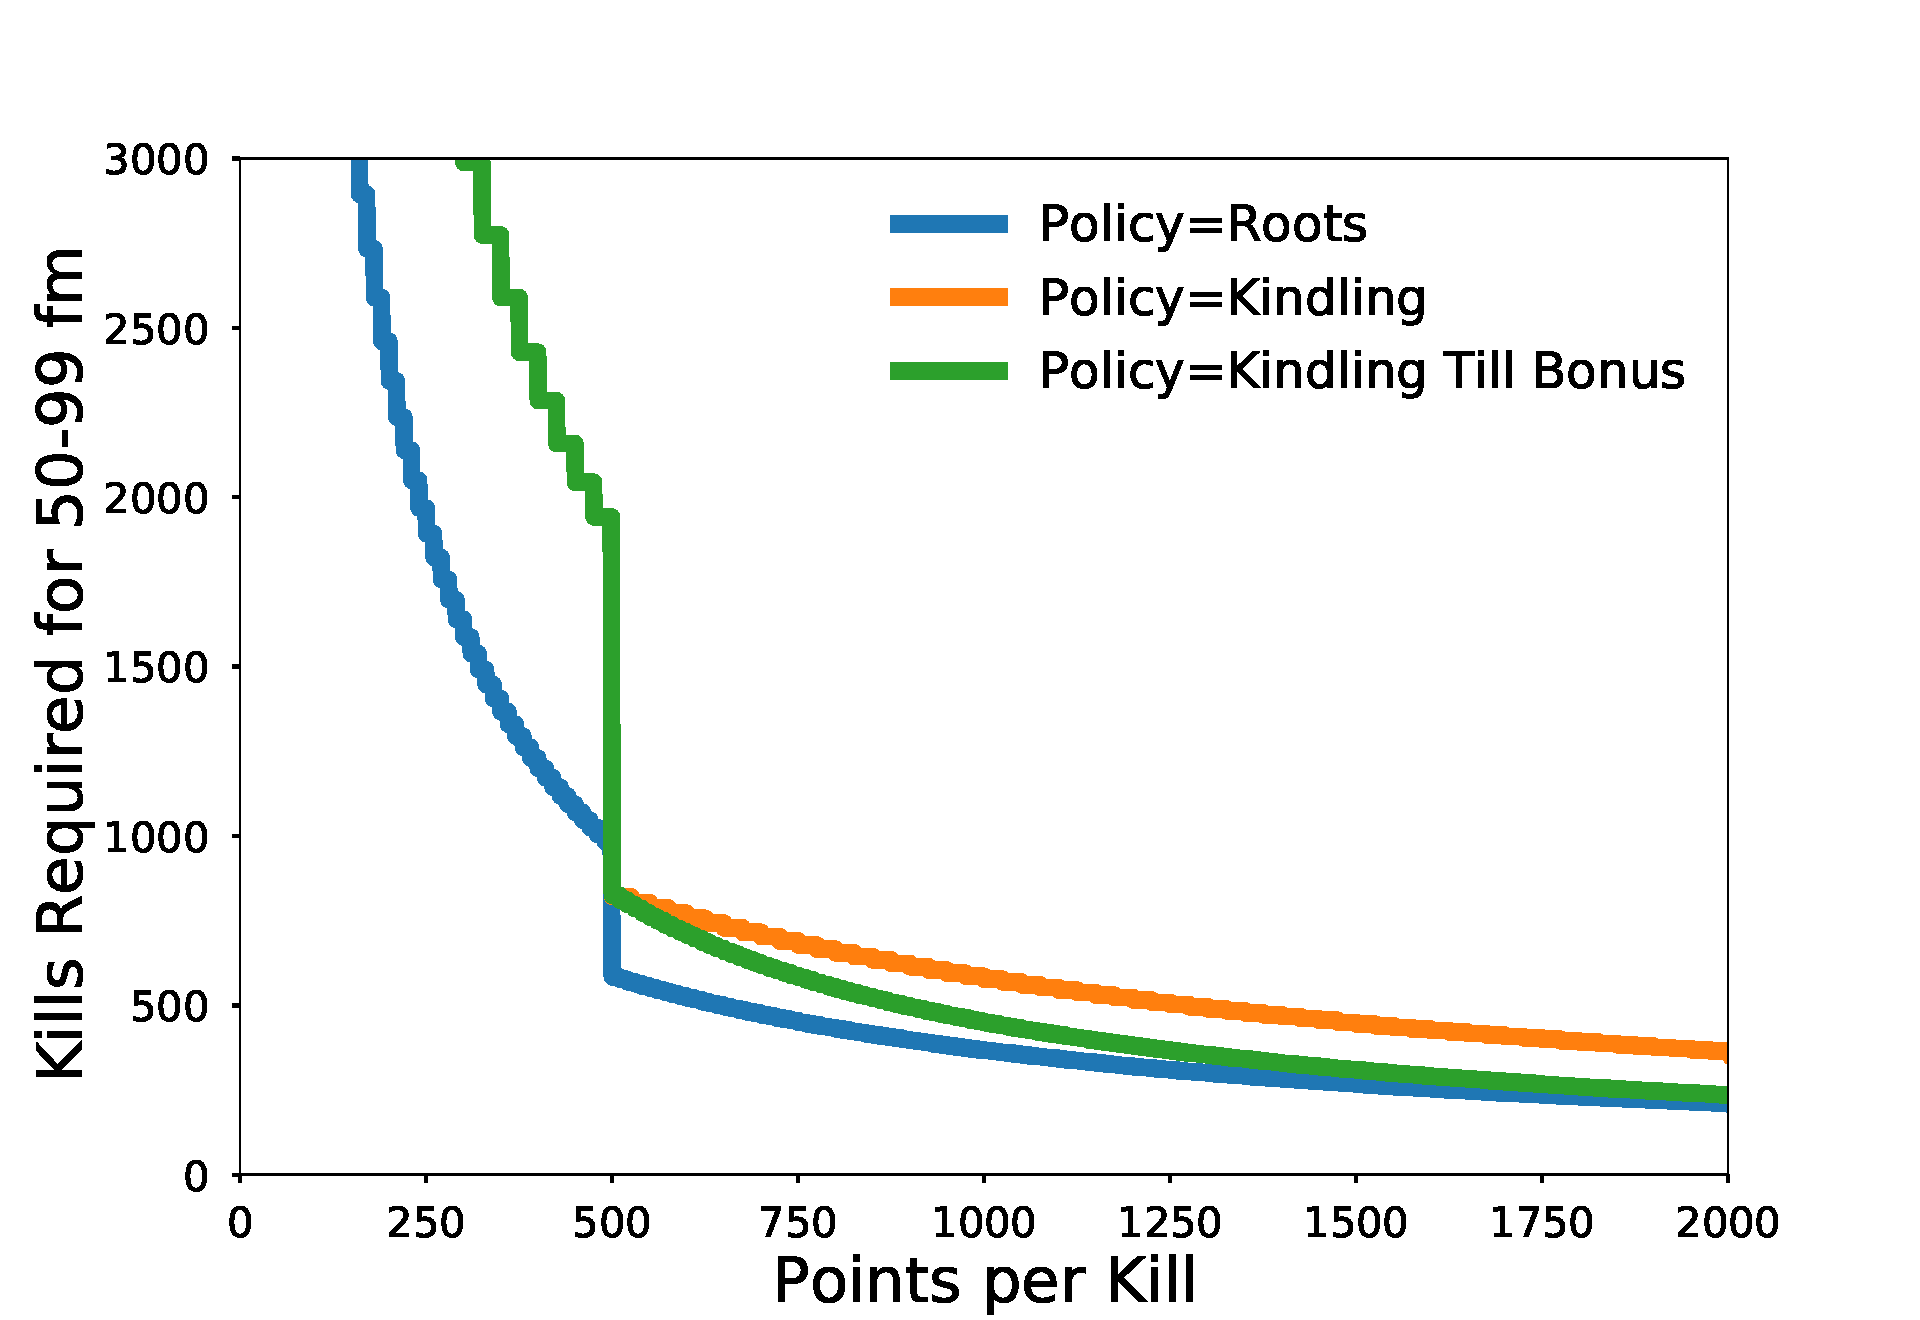
\includegraphics[width=\linewidth]{results/firemaking/policies.pdf}
			\caption{
				A comparison of the kills required to max the firemaking skill at wintertodt for different policies. Before reaching the point threshold, the kindling and kindling-till-bonus policies are equal. Failing to reach the threshold (every game) drastically increases the number of points required, implying that reaching this threshold is essential for players to maximize experience rates. On the other side of the scale, having a very large number of points gives diminishing returns. The roots and kindling policies act as lower and upper bounds for the number of kills, as discussed in the main text.
			}
			\label{fig:wintertodt_policies}
		\end{figure}
		This author reached 99 after 546 kills. Several different playstyles could yield that: 500 points through roots only, 1000 points using kindling only, or 750 points using roughly equal amounts of each - which is anecdotally most similar.

		In this time, the player will be accumulating supply crates as rewards. Each crate gives a certain number of \emph{rolls} on a reward table. The number of rolls given from a crate depends on the points earned in the game, $p$, according to:
		\begin{align}
			\text{Rolls} = \begin{cases}
				\min(1 + p / 500, 28) & \text{if $p \ge 500$} \\
				0 & \text{otherwise},
			\end{cases}
		\end{align}
		where fractional values denote probabilities. Reference~\cite{wiki:wintertodt_supply_crates} provides a (manual) calculator that be used to calculate the value of each roll, and therefore crate. The total value earned after a given number of kills can be calculated as:
		\begin{align}
			\text{Total Value} = \text{Kills} \times \text{Rolls} \times \text{Roll Value}.
		\end{align}
		Based on Fig.~\ref{fig:wintertodt_profit} (bearing in the small number of evaluation points), the value earned increases roughly linearly until about base 70s, after which there are diminishing returns. The value increases exactly linearly as a function of the points earned, since this is simply multiplicative.

		\begin{figure}
			\centering
			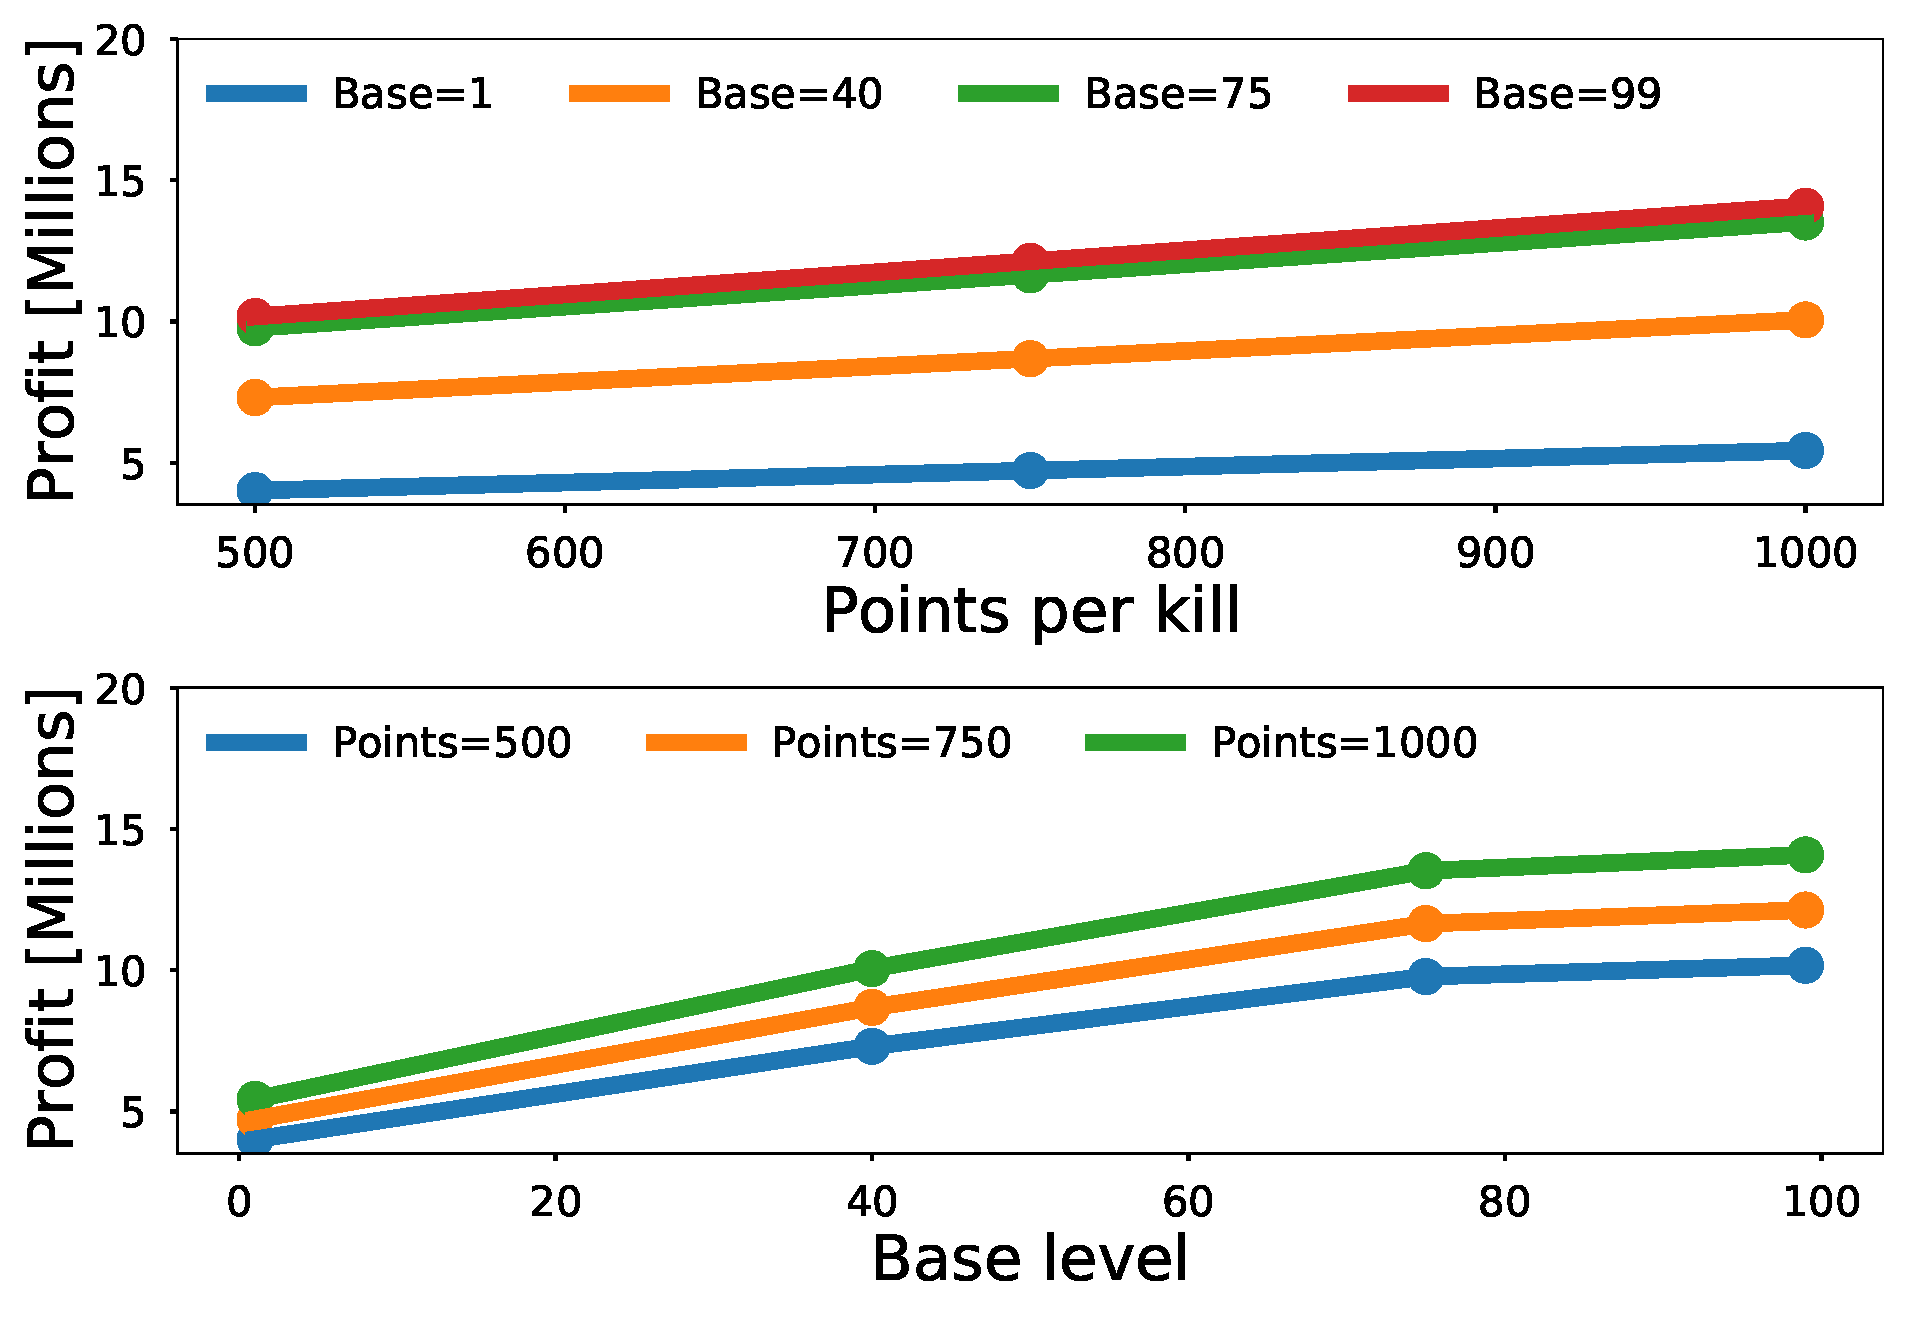
\includegraphics[width=\linewidth]{results/firemaking/profit.pdf}
			\caption{
				The profit a player should expect to gain from 50-99 firemaking, based on their base level, points earned per kill, and only burning roots. The upper panel shows the profit for different base levels. The lower panel shows the profit for different points earned.
			}
			\label{fig:wintertodt_profit}
		\end{figure}

		Reference~\cite{HereticAcinonyx:wintertodt_99_value} provides a case study: with base 1's (except for 46-64 woodcutting) they obtained ~5.5 million gp in 702 kills with 500-800 (estimated) point games, in $\sim$72 hours (which includes initial training and collecting food). 
		It is difficult to discern agreement with the value earned here since prices have since increased/changed since 2016, and the variance in value is unknown. Despite this, the current estimates according to Fig.~\ref{fig:wintertodt_profit} are still around 5 million gp. 702 kills implies closer to 600-700 points mostly using kindling. 5 minute games implies about 58 hours and suggests about 10-15h of preparation, which is reasonable. All in all, these estimates seem to agree with this example.
	
	\section{Future Work}\label{sec:wintertodt_future_work}
		These are possible future avenues to consider:
		\begin{itemize}
			\item Include Action Rates: By including woodcutting, fletching, and burning rates, the action sequence that a player performs could be modeled and optimized (for points or experience). However, the woodcutting rate for Bruma roots is not given.

			\item Food Needed: During the fights the player takes damage that scales with their firemaking and hitpoints level. Some of the attacks are avoidable. Reference~\cite{osrsbox:wintertodt_damage} provides a solid overview of the damage at Wintertodt. However, attack speeds/frequencies don't seem known. If this was known, the total amount of damage taken could be calculated. By accounting for natural regeneration, the amount of food required could be known in advance. This is important since many players train firemaking at Wintertodt right from the start (due to the rewards) and need to collect some preliminary food.

			\item Programmatic Crate Value: More advanced value calculations could be performed if determining crate value could be automated, although it doesn't seem like these equations are given. The wiki team can likely provide insight here. This would also allow the variance and confidence intervals to be determined.

			\item Real Game Duration Data: A stationary recording of wintertodt gameplay could be generated and analyzed to better approximate the distribution of game times. The mean and variance (as a function of player count, which could be approximated by world count) could be used for better estimates.

			\item Large Scale Statistics: The highscores could be analyzed to gain insight into player behaviour. There would have to be some selection criteria to assume a player hasn't gain much experience apart from at Wintertodt. There are standard skills expected for accounts that rush this boss that could be used (although it might be a biased sample). The kill count and total experience can be used to determine the average points per game, and average time spent.

		\end{itemize}

% 		LaTeX Warning: Reference `eq:simplified_recursion' on page 22 undefined on inpu
% t line 1.

% [22]) [23]
% Appendix B.
% (tex/combat/appendix/power_reduction.tex

% LaTeX Warning: Reference `sec:average_damage' on page 24 undefined on input lin
% e 1.